
\chapter{Transmutation of Differential Operators}\label{part1:chap2} %chap 2

Let\pageoriginale $L_1$ and $L_2$ denote two differential operators on the real line
$R$ and $\mathscr{E}^m(x \geq a)$ denote the space of functions $m$
times continuously differentiable in $[ a, \infty)$ furnished with the
  usual topology of uniform convergence of functions together with
  their derivatives upto the order $m$ on each compact subset of $[a,
    \infty)$. Let $E$ be a subspace of the topological vector space
    $\mathscr{E}^m(x \geq a)$. 

\begin{defi*}
  A transmutation of the differential operator $L_1$ into the
  differential operator $L_2$ in $E$ is a topological isomorphism $X$
  of the topological vector space $E$ onto itself (i.e. a linear,
  continuous, one-to-one, onto map), such that 
  $$
  XL_1 = L_2X
  $$
  $X$ is said to transmute the operator $L_1$ into the operator $L_2$
  in $E$ and $L_2 = XL_1 X^{-1}$ on $E$. 
\end{defi*}

\noindent
\textbf{Transmutation in the regular case.} Let $L_1 = D^2_x -q(x),
L_2 = D^2_x$ where $q$ satisfies certain conditions of regularity. The
construction of the transmutation operator in this case depends on the
consideration of certain partial differential equation. 

\begin{prob}\label{part1:chap2:prob1} %problem 1
  To determine $\Phi(x,y)$ in $x \geq a, y \geq a$ satisfying
  $\Phi_{xx}- \Phi_{yy} -q(x) \Phi=0$ with the boundary conditions 
  $$
  \Phi(x, a) = 0 = \Phi (a, y); \Phi_y(x, a) =f(x)
  $$
  This\pageoriginale mixed problem is equivalent to the Cauchy problem if we set
  \begin{align*}
    u(x,y) & = \Phi (x,y)~ \text{ for }~ x \geq a \\
    & = -\Phi (2a-x,y) \text{ for } x \leq a
  \end{align*}
  We set without proof the following proposition.
\end{prob}

\begin{proposition}\label{part1:chap2:prop1} %proposition 1
  \begin{enumerate}[(a)]
  \item If $q \in \mathscr{E}^\circ(R), f \in \mathscr{E}^\circ (x \geq a)$
    with $f(a) =0$, then problem \ref{part1:chap2:prob1} possesses a unique solution which
    is  $(C, 1)$ in $x \geq a, y \geq a$ and satisfies the
    differential equation in the sense of distributions. 
  \item If $q \in \mathscr{E}^1(R)$ and if $f \in \mathscr{E}^2(x \geq
    a)$ with $f(a) =0$, the solution of problem $1$ is $(C, 2)$ in $x
    \geq a, y \geq a$. In the region $y \geq x $(or $x \geq y)$, the
    solution is $(C,3)$. 
  \item If $q \in \mathscr{E}^2 (R)$ with $q' (a) =0$ and $f \in
    \mathscr{E}^3(x \geq a)$ with $f(a) = f''(a) = 0$, then the
    solution $u$ of the problem is $(C, 4)$ in $y \geq a$. [Refer to
      E. Picard, `Lecons sur quelques types simples d' equation aux
      derivces partielles', Paris, Gauthier-VIllars, 1927.] 
  \end{enumerate}
\end{proposition}

With the help of this proposition we prove 
\begin{proposition}\label{part1:chap2:prop2} %proposition 2
  If $q \in \mathscr{E}^2 (R)$ with $q'(a)=0$ and $f \in \mathscr{E}^4
  (x \geq a)$ with $f(a) = f''(a) =0$ then $D^2 Af = ALf$ where $L =
  D^2 = q$ and $A$ is defined by  
  $$
  Af(y) = \frac{\partial}{\partial x} [ \Phi (a,y) ],
  $$
  $\Phi (x,y)$\pageoriginale being the solution of
  problem \ref{part1:chap2:prob1}. 
\end{proposition}

Let $\psi (x,y) = L_x [\Phi (x,y) ] = \frac{\partial^2 \Phi}{\partial
  x^2} - q(x) \Phi$ and $g(x) = L_x f(x)$. As $\Phi$ is $(C, 4)$ by
Proposition \ref{part1:chap2:prop1} $(c)$, and $f \in \mathscr{E}^4 (x \geq a), \Psi (x,y)$
is $(C, 2)$ and $g \in \mathscr{E}^2 (x \geq a )$ with $g (a)
=0$. Replacing $f$ by $g$ in proposition \ref{part1:chap2:prop1}
$(b)$, problem \ref{part1:chap2:prob1} possesses 
a unique solution. We verify below that this unique solution is $\Psi
(x,y)$. 
\begin{align*}
  L_x\Psi - D^2_y \Psi & = L_x L_x \Phi - D^2_y L_x \Phi = L_x[ L_x \Phi
    - D^2_y \Phi ]=0;\\ 
  \Psi (x,a) & = L_x [ \Phi (x,a)] = L_x [0]=0;\\
  \frac{\partial}{\partial y} \Psi (x,y)& = D_y L_x \Phi (x,y) = L_x
  D_y \Phi (x,y) \quad \text{ so that }\\ 
  \Psi_y (x,a) & = L_x D_y \Phi(x,a) = L_x f(x) = g(x);\\
  \Psi (a,y)& = D^2_y [ \Phi (a,y) ]=0.
\end{align*}

Now by definition of $A$, $AL[f(y)] = A.g= \dfrac{\partial}{\partial x}
\Psi (a,y)$ 
$$
\Psi_x (x,y) = D_x L_x \Phi = D^2_y [ \Phi_x (x,y)] \text{ gives }
$$

$\Psi_x (a,y) =  D^2_y [ \Phi_x (x,y)] = D^2_y A f(y)$. Hence we have
proved that $A L = D^2_y A$. 

Computation\pageoriginale of the solution $u(x, y), y \geq a$ of
problem \ref{part1:chap2:prob1}  by using Riemann's
function. \label{page16}
\begin{figure}[H]
  \centering{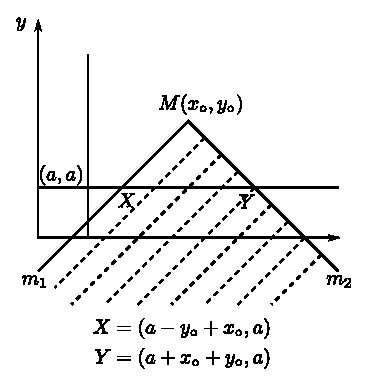
\includegraphics{vol22-figures/fig22-2.eps}}
\end{figure}

Let $K(x, y ; x_0,  y_0)$ be the Riemann's  function defined in the
shaded part of the satisfying the conditions $\dfrac{\partial ^2
  K}{\partial x^2} - \dfrac{\partial^2 K}{\partial y^2} - q^* (x) K =
0$ 

\begin{align*}
  \text{ with } q^* (x) & = q(x) ~\text{if}~ x \geq a\\
  & = q (2 a - x ) ~\text{if}~ x < a 
\end{align*}
and $K$ on $Mm_1 =  K $ on $Mm_2 = - \dfrac{1}{2}$. 

In this case Riemann's method gives 
\begin{align*}
  u (x_0,  y_0) &= \int^{ x_0 + y_0 -a }_{ a - y_0 + x_0} f^* (x) K (x,
  a; x_0, y_0) dx\hspace{2cm}\\
  \text{where } \hspace{1cm} f^* (x) & = f (x) \quad \text{ if } x \geq a \\
  & = - f ( 2a - x ) \quad \text{ if } x \leq a 
\end{align*}
Hence 
\begin{align*}
  A [ f (y_0)] & = \frac{\partial }{\partial
    x_0} u (a, y_0)\\
  & = f (y_0) - 2 \int^{ y_0}_{ a} f (x) \frac{\partial }{\partial x_0} K
  (x, a; a, y_0) dx.    
\end{align*} 

\begin{prob}\label{part1:chap2:prob2}% problem 2
  To\pageoriginale determine the function $\Phi (x, y)$ in $x \geq a, y \geq a $
  satisfying the conditions $\Phi _{xx} - \Phi_{yy} - q (x) \Phi = 0;
  \Phi (a, y ) = 0 ; \Phi_x ( a, y) = g $ where $g \in \mathscr{E}^2
  (y \geq a)$ with $g (a ) = 0 $, and $\Phi (x, a ) =
  0$. Problem \ref{part1:chap2:prob2} ,
  is the same as Problem \ref{part1:chap2:prob1} if in the boundary conditions the lines
  $x = a,  y = a$ are interchanged. If $\Phi$ is the solution of
  Problem \ref{part1:chap2:prob2},  we define a $g (x) =
  \dfrac{\partial}{\partial y} \Phi (x, a)$.  
\end{prob}

\begin{proposition}\label{part1:chap2:prop3}% propositon 3
  If $q \in \mathscr{E}^1 (R)$ and $f \in \mathscr{E}^2 (x \geq a)$
  with $f(a) = 0 $, then $a Af = A a f = f $.  
\end{proposition}

Let $\Phi$ be the solution of Problem \ref{part1:chap2:prob1} and let $g(y) = Af (y) =
\dfrac{\partial}{\partial x} \Phi (a,  y)$. By
Proposition \ref{part1:chap2:prop1} $(b), g$
is $(c, 2)$ in $y \geq a$ and  $g(a) = 0$. Hence $\Phi$ is the
solution of Problem \ref{part1:chap2:prob2} and $a \cdot g(x) =
\dfrac{\partial }{\partial y} \Phi 
(x, a )  = f (x) $. This shows that $a A f = f $. Similarly $A a f =f$.   
 
Proposition \ref{part1:chap2:prop3} together with
Proposition \ref{part1:chap2:prop2} shows that if $q \in
\mathscr{E}^1 (R)$ with $q' (a) = 0$ the map $A$, which is obviously
linear is one-to-one of the space $E = \left\{f / f \in \mathscr{E}^4
(x \geq a), f (a) = f'' (a) = 0\right\}$ onto itself and verifies $ALf =
D^2 Af$. Further in view of the formula for $Af$ on page \pageref{page16} in items
of Riemann's functions, $A$ is continuous on $E$ with the topology
induced by $\mathscr{E}^4 (x \geq a)$. As $E$ is a closed subspace of
the Frechet space $\mathscr{E}^4 (x \geq a ), A$ is a topological
isomorphism. Thus we have proved the existence of the transmutation
operator $A$ in $E$ transmuting $D^2 - q(x)$ into $D^2$ when $q$ is
sufficiently regular.  
 
 We\pageoriginale now consider the problem of transmuting more general differential
 operators $L_i = D^2 + r_i (x) D + s_i (x)~(i = 1, 2)$ into each
 other when $r_i$ and $s_i$ are regular (e. g. $ r_i,  s_1 \in
 \mathscr{E} (R))$.
  
\begin{proposition}\label{part1:chap2:prop4} % propositon 4
   There exists an isomorphism $A_{L_1 L_2}$ of $E$ which satisfies 
   $$
   A_{L_1 L_2}L_1 =  L_2 A_{L_1L_2}.
   $$
\end{proposition} 
 
The proposition will be proved if we prove the existence
of transmutation $X$ of the operator $L_1$ into the operator $D^2 -
q_1$. For then the same method will give a transmutation of $L_2$ into
$L^*_2 = D^2 - q_2$ and each of the operators $D^2 - q_i (i = 1, 2)$
can be transmutated into the operator $D^2$ so that finally we obtain
the required transmutations $A_{L_1 L_2}$ by composing several
transmutations.  
 
Let $R_1 (x) = \int^x _a r_1 (\xi) d \xi $ then the verification of the
following equations is straight forward:  
 $$
L_1 \left[ e^{- \frac{1}{2} R_1 (x) } f(x) \right] =e^{- \frac{1}{2} R_1 (x) } L_1[ f].  
 $$
 Hence we have $Xf (x) = e ^{- \dfrac{1}{2}R_1 (x)} f(x). L^* _1 = D^2 - q_1$ where 
 $$
 q_1 (x)  = \frac{1}{4} r^2 _1 (x) + \frac{1}{2}  r_1 (x) - s _1 (x)
 \in \mathscr{E}.  
 $$

\heading{Application of transmutation to the Mixed Problems of
   differential equations. } 
 
 If\pageoriginale $\Lambda$ is an elliptic operator in$R^n$ ( independent of the
 variable $t$ which corresponds to time) we consider the problem
 of finding a function  $u(x,  t) ~ (x \in R^n,  t$ time) which
 satisfies the differential equation  
 $$
 \Lambda _x (x, t ) + \left(\frac{\partial _2}{\partial t^2} + r (t)
 \frac{\partial}{\partial t} + s(t) \right) u (x, t ) = 0 
 $$
 with the Cauchy data in a bounded domain $\Omega \subset  R^n$ for $
 t = 0$ and also on the hemicylinder $\Omega^* \times [t \geq 0]$
 where $\Omega^*$ denotes the frontier of $\Omega$. In this problem
 the variable $x$ which corresponds to space and the variable $t$
 which corresponds to time are strictly separated. Suppose that $A_t$
 is a transmutation in the variable $t$ which transmutes
 $\dfrac{\partial ^2}{\partial t^2} + r(t) \dfrac{\partial }{\partial
   t}+ s(t)$ into $\dfrac{\partial^2}{\partial t^2}$ and let $V(x, t) = A_t u(x, t )$ when $u (x, t )$ is the
 solution of the differential equation. Then applying $A_t$ to the
 left hand member of the equation we have  
 $$
 \displaylines{\hfill 
 A_t \Lambda _x u (x, t) + A_t (\frac{\partial ^2}{\partial t^2} +
 r(t) \frac{\partial}{\partial t}+ s (t )) u (x, t) = 0 \hfill \cr
 \text{i.e.,}\hfill \Lambda_x v (x, t) + \frac{\partial ^2 v (x,
   t)}{\partial t^2} = 0\hfill }
$$
 and $v(x, t)$ satisfies Cauchy's data i.e., by means of the
 transmutation, consideration of the gives equation is reduced to the
 consideration of the wave equation.  
 
